\documentclass[conference]{IEEEtran}
\IEEEoverridecommandlockouts
% The preceding line is only needed to identify funding in the first footnote. If that is unneeded, please comment it out.
\usepackage{cite}
\usepackage{amsmath,amssymb,amsfonts}
\usepackage{algorithmic}
\usepackage{graphicx}
\usepackage{textcomp}
\usepackage{xcolor}
\usepackage{multirow}

\def\BibTeX{{\rm B\kern-.05em{\sc i\kern-.025em b}\kern-.08em
    T\kern-.1667em\lower.7ex\hbox{E}\kern-.125emX}}
\begin{document}

\title{Classification of Brain Tumors by Image Processing and Ensemble Learning\\}

\author{\IEEEauthorblockN{1\textsuperscript{st} Hakan Tekgul}
\IEEEauthorblockA{\textit{Electrical and Computer Engineering} \\
\textit{Georgia Institute of Technology}\\
Metz, France \\
htekgul3@gatech.edu}
\and
\IEEEauthorblockN{2\textsuperscript{nd} Jad Sinno}
\IEEEauthorblockA{\textit{Electrical and Computer Engineering} \\
\textit{Georgia Institute of Technology}\\
Metz, France \\
jsinno3@gatech.edu}
\and
\IEEEauthorblockN{3\textsuperscript{rd} Madhur Gupta}
\IEEEauthorblockA{\textit{Electrical and Computer Engineering} \\
\textit{Georgia Institute of Technology}\\
Metz, France \\
mgupta325@gatech.edu}
}

\maketitle

\begin{abstract}
When diagnosed at a late stage, brain cancers and tumors provide very short life expectancy and a high mortality rate because of their aggressive nature. In order to diagnose and detect the tumor on the brain at the earliest stage possible, various medical imaging techniques such as Computed Tomography (CT) or Magnetic Resonance Imaging (MRI) are used. Unfortunately, the diagnosis and treatment of the tumor depends highly on the physician’s medical knowledge. Hence, many different systems have been proposed in the past decade to automatically detect brain tumors by using machine learning. One major problem with these approaches is the fact that they usually need lots of training data (MRI Scans).  

In this project, we detect brain tumors from MRI images with a limited amount of training data, around 120 images. Specifically, we use an ensemble learning approach that is based on Support Vector Machines (SVM). After applying image processing techniques such as low-pass filtering to all the images, the most common prediction from different SVM classifiers is chosen for a testing image. Validation accuracies are used to select the best image processing techniques and their optimal parameters. Our experimental results suggest that the Ensemble Classifier achieves an accuracy of 87\% with low time complexity.
\end{abstract}

\begin{IEEEkeywords}
Brain Tumor, Image Classification, Ensemble Learning, Medical Imaging, SVM
\end{IEEEkeywords}

\section{Introduction}\label{intro}
\subsection{Motivation}
% Explain the motivation behind project and goal of project
Brain cancers and tumors affect the life of humans negatively, as abnormal growth of brain cells damage the functioning of the brain and might even lead to death. With increased usage of cell phones, the incidence rate of brain tumors is predicted to rise rapidly \cite{b1}. Furthermore, the mortality rate of brain cancers have also been increasing constantly in the past decade \cite{b2}. In order to reduce the mortality rate and treat brain tumors, diagnosis should be done in the earliest stage possible. 

Medical imaging is used to diagnose and visualize different types of tumors in the human body. Various medical imaging techniques such as CT Scan, MRI, or X-Ray is used in hospitals for diagnosis. Magnetic Resonance Imaging (MRI) is generally used for brain tumor diagnosis as it shows the inside of the brain with contrast \cite{b7}. With the use of MRI, brain tumors are identified as soon as possible by many physicians. However, some MRI scans are hard to read and there is a chance that physicians can make a mistake during diagnosis. When a physician decides that a tumor in the brain does not exist but in reality there is a tumor, a false negative diagnosis occurs and such diagnosis can be catastrophic for the patient. Hence, many different systems have been proposed in the past decade that automatically identifies brain tumors in an MRI scan. Even though most of these approaches have good accuracy and results, they usually need a huge number of training data and computation resources. Therefore, new approaches for brain tumor classification must be considered. 

In this work, we propose to detect brain tumors from MRI images with a limited amount of training data. Specifically, we use image processing and ensemble learning through Support Vector Machines (SVM) to classify whether an MRI scan has a tumor or not. Our main goal in this study is to maximize the classification accuracy and minimize the number of false negatives. We use different image processing techniques, inluding Low-Pass Filter (LPF), High-Pass Filter (HPF), Median Filter (MF), and Low-Pass - High-Pass Filter (LPF+HPF). Then, we apply different machine learning algorithms such as k-NN, SVM, and Neural Networks (NN). To summarize, we make three main contributions in this paper:
\begin{itemize}
  \item We apply different image filters to MRI scans and analyze the best processing technique for tumor detection.
  \item We experiment with three different machine learning algorithms and state their accuracy for differrent image processing techniques.
  \item We propose an ensemble learning approach that successfully identifies a tumor in the brain with a minimum number of false negatives. 
\end{itemize}
Our experimental results suggest that LPF+HPF is the best filter to use for tumor detection, with an average classification accuracy of 84\%. Additionaly, we observed that Support Vector Machines (SVM) gives the optimal results in terms of classification. Finally, our ensemble learning approach that is based on different filters and Support Vector Machines outputs a classification accuracy of 87\% and a 2\% false negative rate. 

\subsection{Related Work} 
% Discuss some related work. Provide around 5-6 projects about tumor classification and summarize their improvements/results
% DO NOT FORGET TO CITE
The development of brain tumor recoginition has been increasing in the past decade. Many appraoches have been proposed that build different models for MRI scan classification. Some approaches use image processing techniques, whereas some approaches are solely focused on deep learning to identify tumors. Some of the related work to our project is presented below. 

Firstly, Praveen \cite{b3} introduced the use of image processing and segmentation for the problem of tumor detection. Different imaging filters such as median filter, wiener filter are used to process images and different edge detection and feature extraction techniques are used for classification. Then, Gaikwad et. al \cite{b4} experimented with dimensionality reduction of MRI images using Principal Component Analysis (PCA) and developed a Probabilistic Neural Network for tumor classification. 

Apart from image processing or segmentation, Ari et. al \cite{b5} used deep learning to classify brain tumors by focusing on extreme learning machine local receptive fields (ELM-LRF) based tumor classification. Their work showed very promising accuracy results. Similarly, Seetha et. al \cite{b6} used convolutional neural networks with deep architecture and small kernels to classify brain tumors. By setting the weights of neurons to small values, their results were also very promising. The only problem with deep learning approaches is the fact that they usually need lots of training data. 

As compared to these works, we experiment with a wide range of image processing techniques and we analyze the best imaging filter to use for tumor detection. Even though our accuracy value is not very high compared to works that used deep learning, we propose a classifier that can work well with limited amount of training data. To the best of our knowledge, this project is the first to apply ensemble learning for tumor identification. Finally, this work is also the only one that tries to minimize false negatives as well as accuracy, and discuss the results. Hence, we believe our contribution to brain tumor classification is significant.


\section{Methodology}\label{method}
% Put the flowchart here 
\begin{figure}[h]
\centering
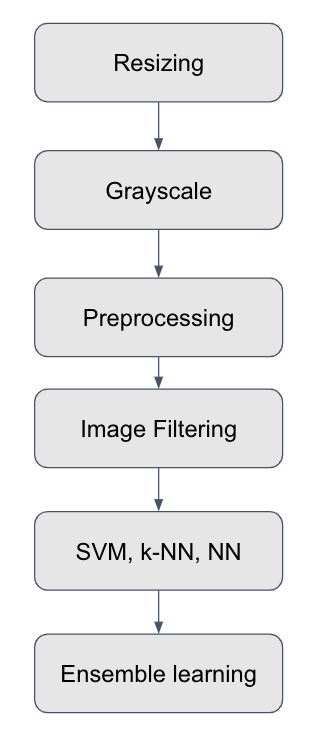
\includegraphics[scale=0.4]{flowchart}
\caption{Flowchart of the project that summarizes our process for our experiments.}
\end{figure}
% Explain our methodology behind the project
% Talk briefly about resizing and grayscale. Maybe put the graph on image sizes? 

For this project, we used an MRI Scan dataset that has a total of 255 images. The dataset is balanced, where there are 156 positive images and 99 negative images. From the 255 images, 70\% is used for training and 30\% is used for testing. After that, all the images are resized to a certain size and each image is converted to grayscale. This was because the MRI scans usually consist of black and white pixels and RGB colors does not contribute to identification of tumors. Note that the methodology behind this project is shown in Figure 1.

\subsection{Image Preprocessing}
% Describe the equalization and contrast images
% Add histograms, equalized and contrast image examples, visualize sigmoid etc. 
To be fed into the classifier, the images had to be resized to a common size. In our case, we resized them all to $350\times300\: px$ around which most images were distributed (Figure 2). The method used is either downsampling for downscaling or upsampling the images using bicubic interpolation for upscaling.
\begin{figure}[h]
\centering
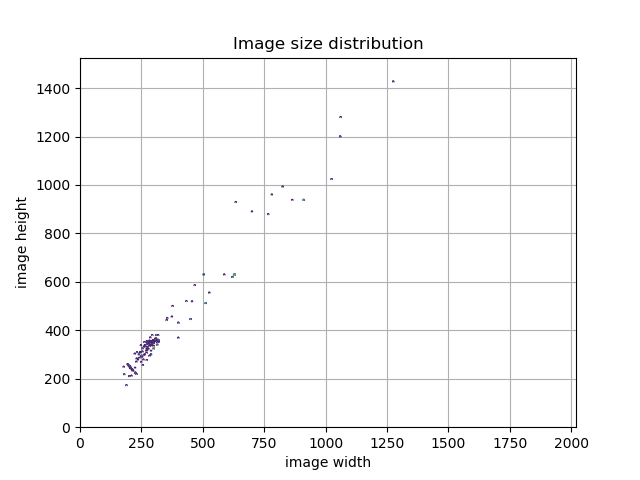
\includegraphics[scale=0.5]{figures/Image_size_distribution.png}
\caption{Original image size distribution in pixels.}
\end{figure}

From this homogeneous dataset, two sub-datasets were created : the first one adds contrast to the images, the second one equalizes the histograms.\\
\paragraph*{Contrast addition}
In the following example (Figure 3), the tumor stands out by the luminance difference with healthy brain tissue. Thus our hypothesis is that adding contrast can help emphasizing the even more the tumor. The method used is a sigmoïd transformation : for every pixel $x \in [0;255]$, $$x\leftarrow x\times \frac{1}{1+e^{-0.02(x-127)}}$$
\begin{figure}[h]
\centering
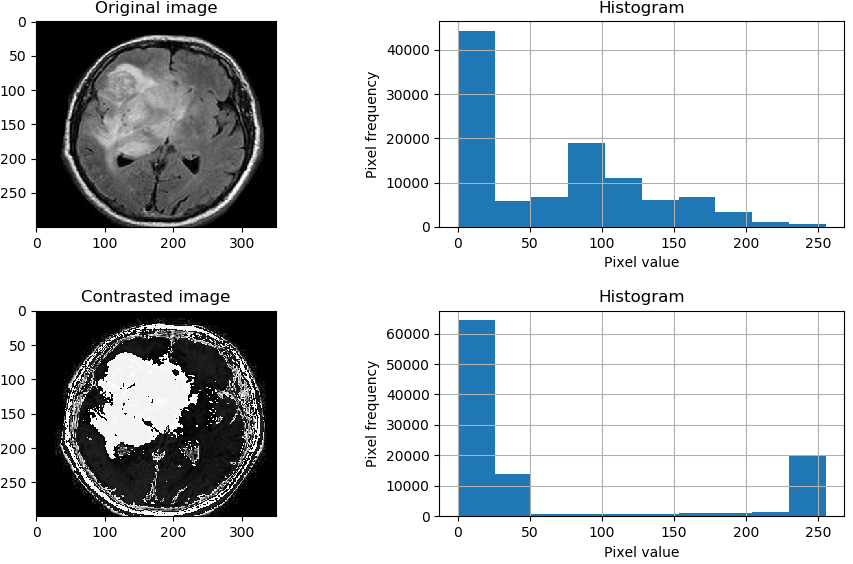
\includegraphics[scale=0.33]{figures/Contrasting.png}
\caption{Sample image of a brain having tumor and associated histogram before and after adding contrast.}
\end{figure}

\paragraph*{Equalization}
In the following example (Figure 4), there is no clear tumor (and in fact there is no tumor, but we don't know it beforehand), and most pixels are concentrated around a certain gray value, making it difficult to distinguish details. Thus our hypothesis is that histogram equalization can help distinguishing details, for example distinguishing a tumor when its luminance is close to healthy brain tissue. \\
\begin{figure}[h]
\centering
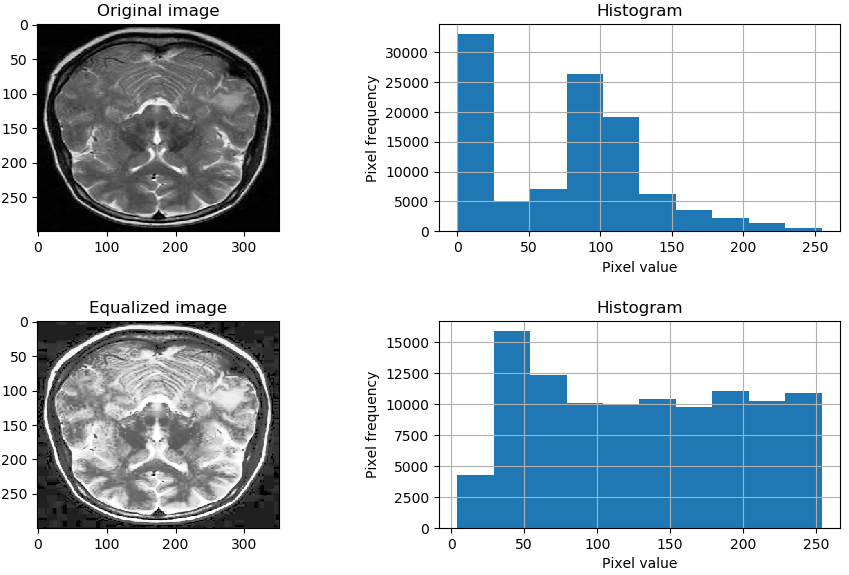
\includegraphics[scale=0.33]{figures/Equalizing.png}
\caption{Sample image of a brain without tumor and associated histogram before and after equalizing histograms.}
\end{figure}

\subsection{Image Filtering}
% Describe and explain the different filters 
For image filtering, a low pass filter (LPF) is used to smooth the images and remove the high frequency components and noise in the images. LPF is applied with various sigma values to the contrast and equalized images. Additionally, a high pass filter (HPF) is used with various sigma values on the contrast and equalized images. HPF helped us to concentrate on the high frequency regions in MRI scans and we assumed that the tumors in the images had high frequency. Figure 5 shows example MRI scans after LPF and HPF filtering, whereas Figure 7 presents the general structure and visualization of both filters. 

\begin{figure}[h]
\centering
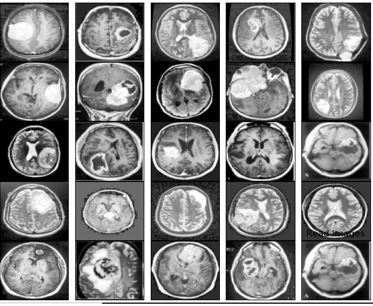
\includegraphics[scale=0.43]{figures/lpf.JPG}
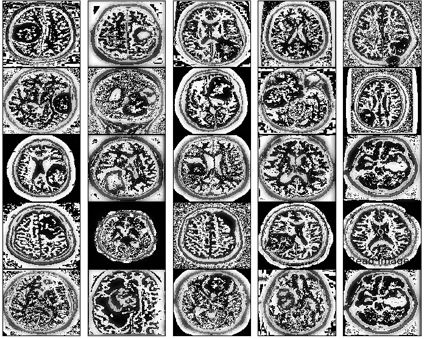
\includegraphics[scale=0.39]{figures/hpf.JPG}
\caption{LPF(sigma=2) and HPF(sigma=10) applied on equalized image examples respectively.}
\end{figure} 

We also combined the above two filters to filter the images in our dataset. Specifically, we first applied the low-pass filter and then the high-pass filter (LPF+HPF) as it helped us to remove the noise in the images and then perform the classification on the relatively high frequency content in the image. Finally, we used the Median Filter to filter the images as it ouputs good quality images for the classification part of our project. The filter takes the median of the neighborhood of each of the pixels in the image and replaces the specified pixel by that value. Example images after applying LPF+HPF and Median Filter is shown in Figure 6.

% Provide examples of filtered images (one image from each filtering is fine)
\begin{figure}[h]
\centering
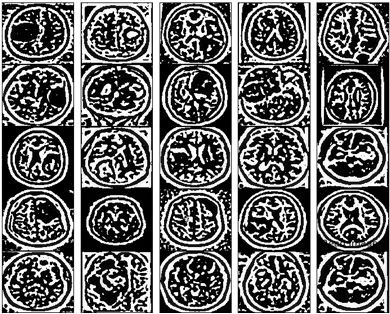
\includegraphics[scale=0.40]{figures/lpf_hpf.JPG}
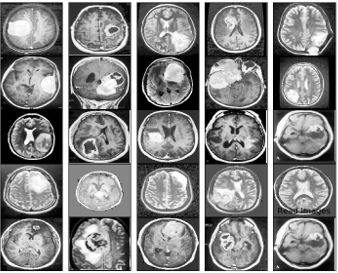
\includegraphics[scale=0.46]{figures/median.JPG}
\caption{LPF+HPF(sigma=5) and Median filter (sigma)=5) applied on equalized images examples respectively.}
\end{figure}

% Note that, the filters used are GAUSSIAN --> would be nice to visualize the filters in a graph
\begin{figure}[h]
\centering
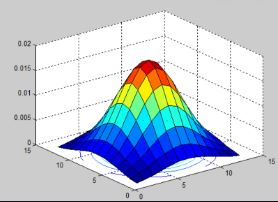
\includegraphics[scale=0.4]{figures/lpf_filter.JPG}
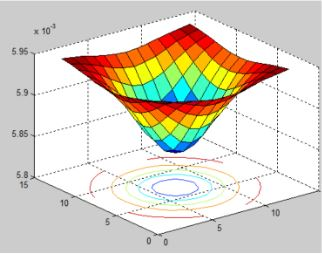
\includegraphics[scale=0.32]{figures/hpf_filter.JPG}
\caption{Visualization of Gaussian LPF and HPF respectively.}
\end{figure}

\subsection{Machine Learning}
% Briefly describe the machine learning algorithms 
After creating the contrasted, equalized versions of the dataset and applying different image filters, classification experiments are conducted by applying three different machine learning algorithms. As stated before, k-Nearest Neighbors (kNN), Support Vector Machines (SVM), and Artificial Neural Networks (NN) are applied on our data. k-NN is chosen because of its simplicity and the fact that our images are not that complex in nature. SVM, on the other hand, is selected as a machine learning algorithm because it can work very well with low amount of training data and it handles outliers very well. Finally, because image classification is usually done with Neural Networks, we chose NN as the last algorithm. 

% Cross validation
After choosing the algorithms, the dataset is split into training, validation, and testing. As stated before, 70\% of data is used for training and 30\% of training set is used for validation. Then, all the specified machine learning algorithms are applied to the training set and cross-validation approach is used to tune the parameters of each algorithm. After the optimization of the classifiers, accuracy results are collected for different classifiers, different image filters, and their different sigma values. Such results are presented in section 3. 

% Ensemble Learning
Finally, best 8 classifier/filter/sigma combinations that had the maximum but different accuracies are selected for ensemble learning. Ensemble learning is applied because some of the classifiers had overfitting and there was a need to generalize the data better. At the end, the most common prediction from the 8 classifiers is taken as the final result. In the case of a tie, the classifier predicts a positive instance to lower the number of false negatives. Figure 8 shows our final classifier with best classifier and sigma selections.

\begin{figure}[h]
\centering
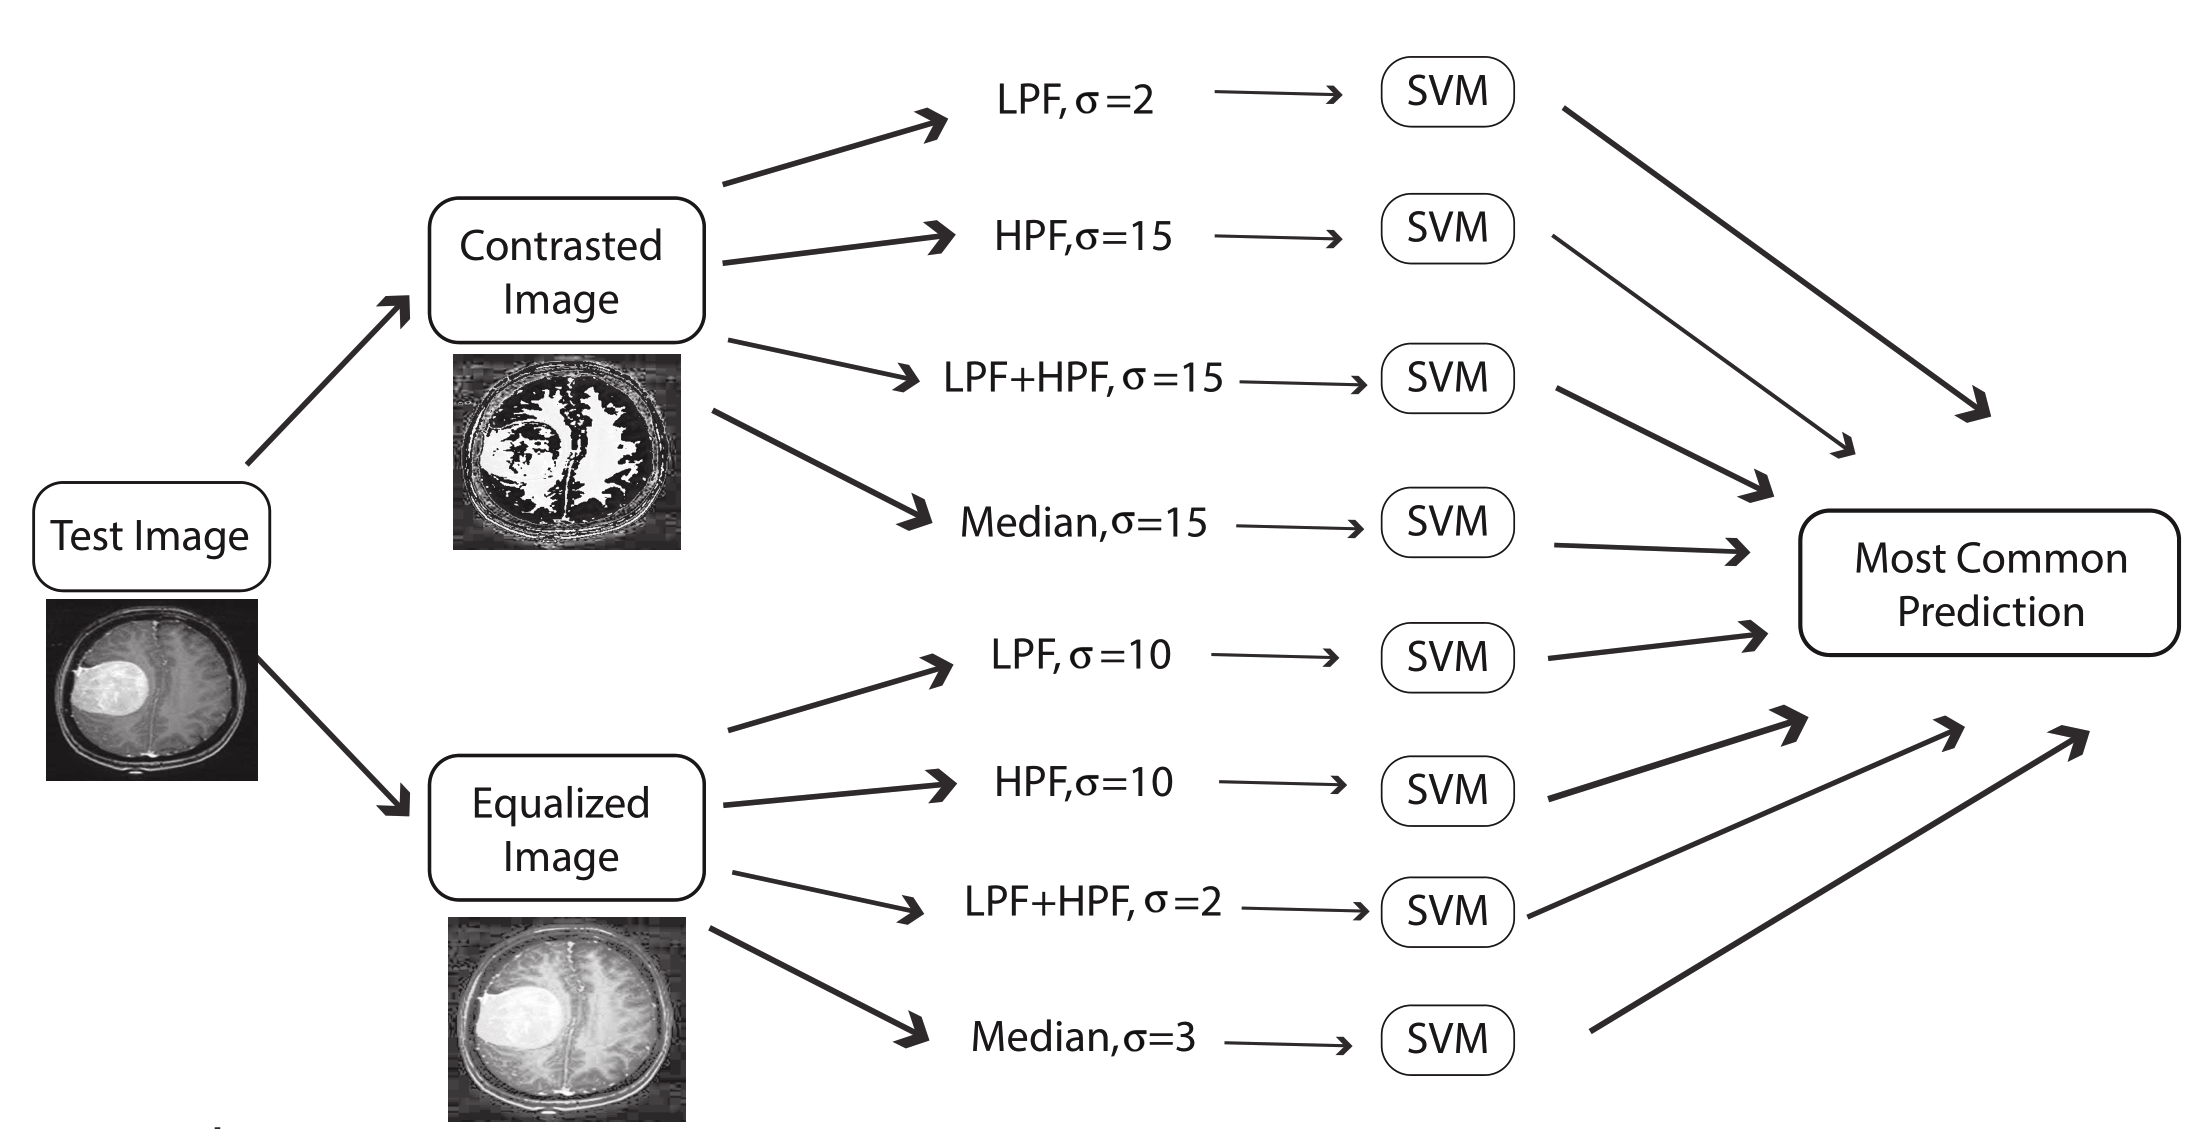
\includegraphics[scale=0.1]{final_classifier_diagram}
\caption{Final classifier diagram for brain tumor identification that is based on ensemble learning.}
\end{figure}

\section{Experimental Results}\label{results}
Tables 1 through 3 present and summarize our experimental results for this project. As stated, we experimented with a wide range of imaging filters with different sigma values. For each sigma value, accuracy result from imaging filters are collected from both contrasted and equalized versions of MRI images. The first row of accuracy values in each table provides contrast image values, whereas the second rows show the accuracy values of equalized images. 

Experimental results suggest that applying a low-pass filter and a high-pass filter (LPF+HPF) outputted the best accuracy values among all classifiers on average. Specifically, SVM classifier had an average of 0.8247 from LPF+HPF technique among all sigma values and both contrasted and equalized images. The worst filter in terms of accuracy among all classifiers was the median filter, with an average of 0.7353. 

Other than that, the results from different classifiers suggest that SVM is the best classifier for all different image processing techniques and sigma values, with an average of 0.8111. The worst classifier, in terms of accuracy, is Neural Network (NN) classifier, with an average of 0.7349. 

Finally, the results suggest that, low sigma values benefit the accuracy score for LPF, whereas high sigma values benefit the accuracy score for HPF processing technique. For LPF+HPF and Median Filter, all the sigma values show similar results across all classifiers. An evaluation of our results and a thorough analysis is presented in the next section. 

\begin{table}[h!]
\centering
\caption{SVM results for different filters and sigma values.}
\label{table:1}
\begin{tabular}{ |p{1.4cm}||p{1.1cm}|p{1.3cm}|p{1.1cm}|p{1cm}|  }
\hline
 SVM & LPF &LPF+HPF &HPF & Median\\
 \hline
 \multirow{2}{*}{Sigma = 2} &0.8289 &0.8157& 0.75&0.7916\\ 
 &0.8157	&0.8421&	0.77&0.8151\\
\hline
\multirow{2}{*}{Sigma = 5}  & 0.8289&	0.8354	&0.71	&0.8026\\
&  0.8289& 0.8289	& 0.7894	&0.8026\\
\hline
\multirow{2}{*}{Sigma = 10}  &	0.8157	&0.8157&	0.8157	&0.8026\\
&	0.8421	& 0.7891&0.8373	& 0.8026\\
\hline
\multirow{2}{*}{Sigma = 15} &	0.8157&	0.8421&	0.8555&	0.8157\\
& 0.8157&	 0.8289&	  0.8157&  0.7894\\
 \hline
 \multirow{2}{*}{Avg. accuracy} &0.8223 & 0.8273 & 0.7828 & 0.8031 \\
&0.8256 & 0.8223 & 0.8031 & 0.8024 \\
\hline
\end{tabular} \\
\end{table}

\begin{table}[h!]
\centering
\caption{KNN results for different filters and sigma values.}
\label{table:2}
\begin{tabular}{ |p{1.4cm}||p{1.1cm}|p{1.3cm}|p{1.1cm}|p{1cm}|  }
\hline
 KNN & LPF &LPF+HPF &HPF & Median\\
 \hline
 \multirow{2}{*}{Sigma = 2} & 0.6184 & 0.8026 & 0.8151  & 0.6050 \\ 
& 0.7894 &  0.8026 & 0.7243 & 0.7894 \\
\hline
\multirow{2}{*}{Sigma = 5} & 0.6728 & 0.8151 & 0.789  & 0.6050  \\ 
 &0.7368 &  0.8151 & 0.8289 &  0.8026 \\ 
\hline
\multirow{2}{*}{Sigma = 10} & 0.7105 & 0.8151 & 0.7140  & 0.5526  \\
& 0.7368 &  0.8289 & 0.7519 &  0.7763 \\
\hline
\multirow{2}{*}{Sigma = 15} & 0.7763  & 0.8233  & 0.6766 & 0.6050 \\
& 0.7336 &  0.8684 & 0.7243 &  0.7763 \\
 \hline
 \multirow{2}{*}{Avg. accuracy} &	0.6945 & 0.8140 & 0.7486 & 0.5919   \\
&0.7492 & 0.8288 & 0.7574 & 0.7862 \\ 
\hline
\end{tabular}
\end{table}

\begin{table}[h!]
\centering
\caption{NN results for different filters and sigma values.}
\label{table:3}
\begin{tabular}{ |p{1.4cm}||p{1.1cm}|p{1.3cm}|p{1.1cm}|p{1cm}|  }
\hline
NN & LPF &LPF+HPF &HPF & Median\\
 \hline
 \multirow{2}{*}{Sigma = 2} & 0.8026  & 0.7894  & 0.6315& 0.7763  \\
 & 0.7763 &  0.8026 & 0.7243 &  0.7894 \\
\hline
\multirow{2}{*}{Sigma = 5} & 0.7763 & 0.7894 & 0.6315& 0.7376  \\
 &  0.7519 & 0.8026 &  0.7376 & 0.7376 \\
\hline
\multirow{2}{*}{Sigma = 10}  & 0.6315& 0.8032  & 0.6982 & 0.7376\\
 & 0.7368 & 0.7894 & 0.7376 & 0.7376 \\
\hline
\multirow{2}{*}{Sigma = 15} & 0.6050 & 0.7763 & 0.7336 & 0.6315 \\
&  0.7763 &  0.7763 & 0.7336 &  0.6315 \\
 \hline
  \multirow{2}{*}{Avg. accuracy} &0.7039 & 0.7934  & 0.6649 & 0.7076  \\
&0.7603 & 0.79273 & 0.7333 & 0.7240   \\
\hline
\end{tabular}
\end{table}
% Provide experimental results here
% Provide 3 different tables --> cluster all k-NN results together into one table, same for SVM and NN

\section{Analysis of Results}\label{analysis}
% Detailed analysis of all results and process
Since the goal of this paper is to not only propose a classifier that has high accuracy of classification but also to select the best image processing technique for brain tumor identification, there is a need to discuss and evaluate our results. 

To start with, as stated, the best image filtering technique among all three classifiers is LPF+HPF. LPF+HPF is actually a popular choice of processing for medical images as it is very helpful to smooth the images and focus on the high frequency content [REF]. Usually, medical image processing is used for diagnosis and identification of certain abnormal tissues in different images. In such a case, LPF+HPF removes the bright parts of the image except the high frequency content such as a tumor and it can be really helpful for classification. Additionally, LPF+HPF images from Figure 6 suggests that the output images are very different from original MRI scans and tend to capture the structure of the brain and kind of segment the brain tissue from background pixels. This is very helpful for the sake of our project as our classifier would be able to focus solely on brain tissue and try to detect abnormal, big cancer tissues in images. Hence, it definitely makes sense that LPF+HPF was the dominant image filtering technique for our experiments. However, we did not only focus on LPF+HPF when building our final classifier as our training data was limited and we wanted to increase the generalization of our data by picking the best validation accuracy scores of different image filter, sigma, and classifier combinations. 

It is also observed that Median Filter outputted the lowest accuracy values, which makes sense as median filter is generally used to remove significant noise from images and our data does not have that much noise. LPF and HPF, on the other hand, provided various accuracy results among different classifiers. Figure 5 example images of LPF show that LPF outputs images that are very similar to original MRI scans but has smooth edges and is a little blurry. Hence, LPF does not change the structure or appearance of original images but enhances the result of classification. HPF, however, outputs significantly different images compared to original scans as low frequency content gets removed and the tumor is more visible. HPF is helpful for segmenting the large size tissues of brain and certainly helps with our classification results. 

Furthermore, it is observed that LPF benefits from low sigma values for tumor identification. This is because a low-pass filter with very high variance can easily remove the high frequency content and the tumor itself from MRI scans and smooth the image unnecessarily. Hence, a low-pass filter with small variance would only smooth the edges of the skull and remove some noise. As for HPF, high sigma values are dominant as HPF helps to identify and keep the high frequency content in MRI scans. Figure 5 HPF images suggest that the tumor regions are much more dominant compared to the original MRI images. When the dominant LPF+HPF results are analyzed, similar accuracy scores are observed for various sigma values. This makes sense as LPF+HPF with small sigma is already a very significant change for the images and a high sigma would not change the images that much or affect the tumor classification. A similar argument can also be constructed for Median Filter images, as a very high variance would not change the result of classification because of the lack of noise in images. 

Finally, it is important to discuss why some classifiers worked better than others after the application of image processing techniques. As stated, SVM classifier turned out to be the best classifier in terms of accuracy and false negatives. We believe the reason for this is our limited training data as SVM tends to perform well with a low amount of training data. SVM focuses on maximizing the margin between the support vectors and creates the most optimal decision boundary. By using a Gaussian RBF kernel for our SVM classifier, we made sure that our data is close to being linearly separable. Additionally, Figure 9 shows the learning and validation curves of SVM classifier for LPF+HPF filtering. The learning curve suggests that there is some sort of overfitting with our limited training data, but addition of training examples definitely increases the validation score. Hence, we can argue that different methods such as data augmentation could be used to increase training data, which would also increase the validation accuracy. Instead of data augmentation, we used image processing and ensemble learning to increase the final accuracy. The validation curve suggests that a larger-margin hyperplane is better for tumor identification. 

\begin{figure}[h]
\centering
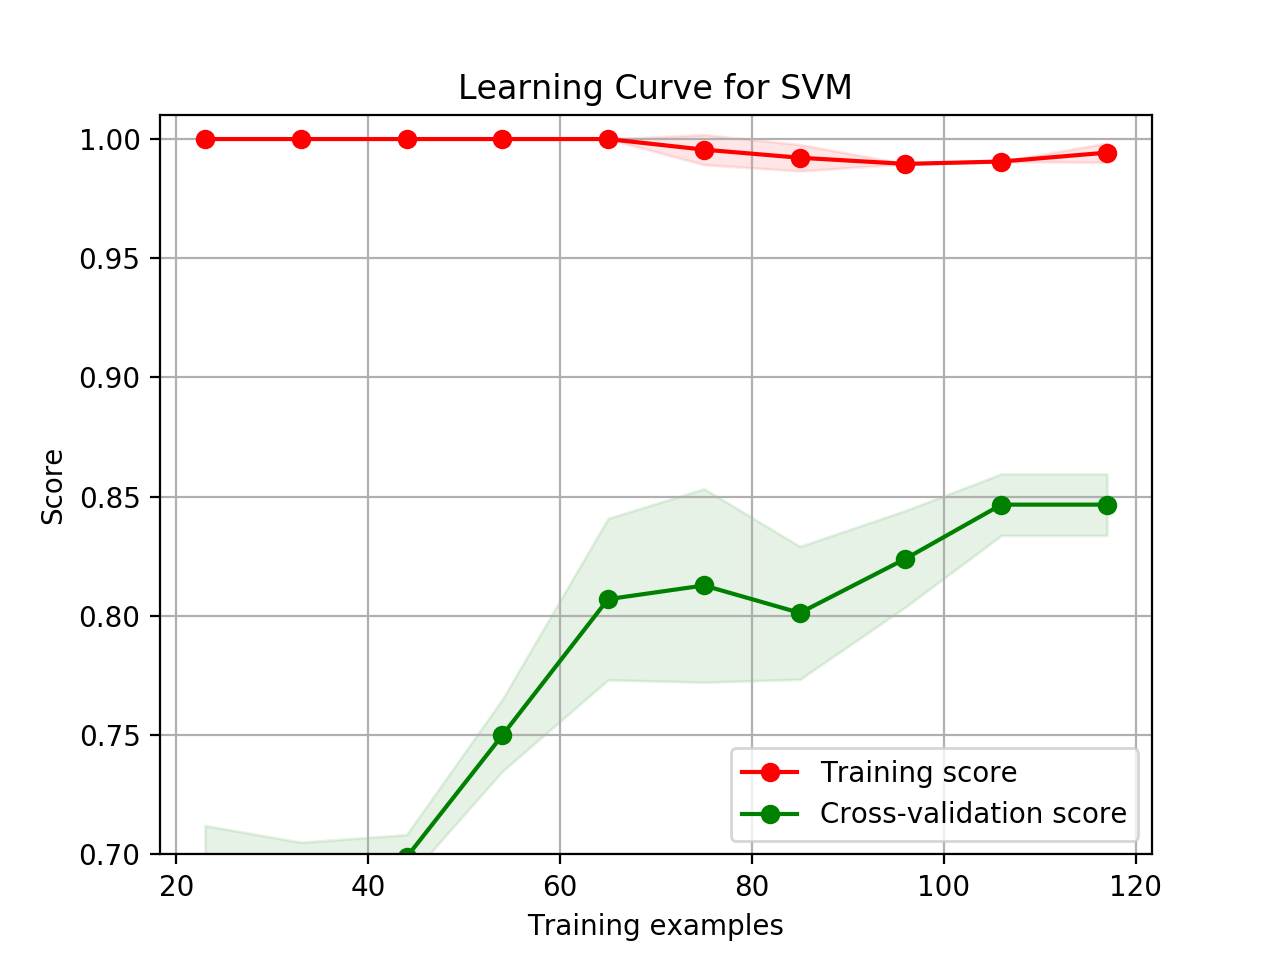
\includegraphics[scale=0.26]{learning_curve}
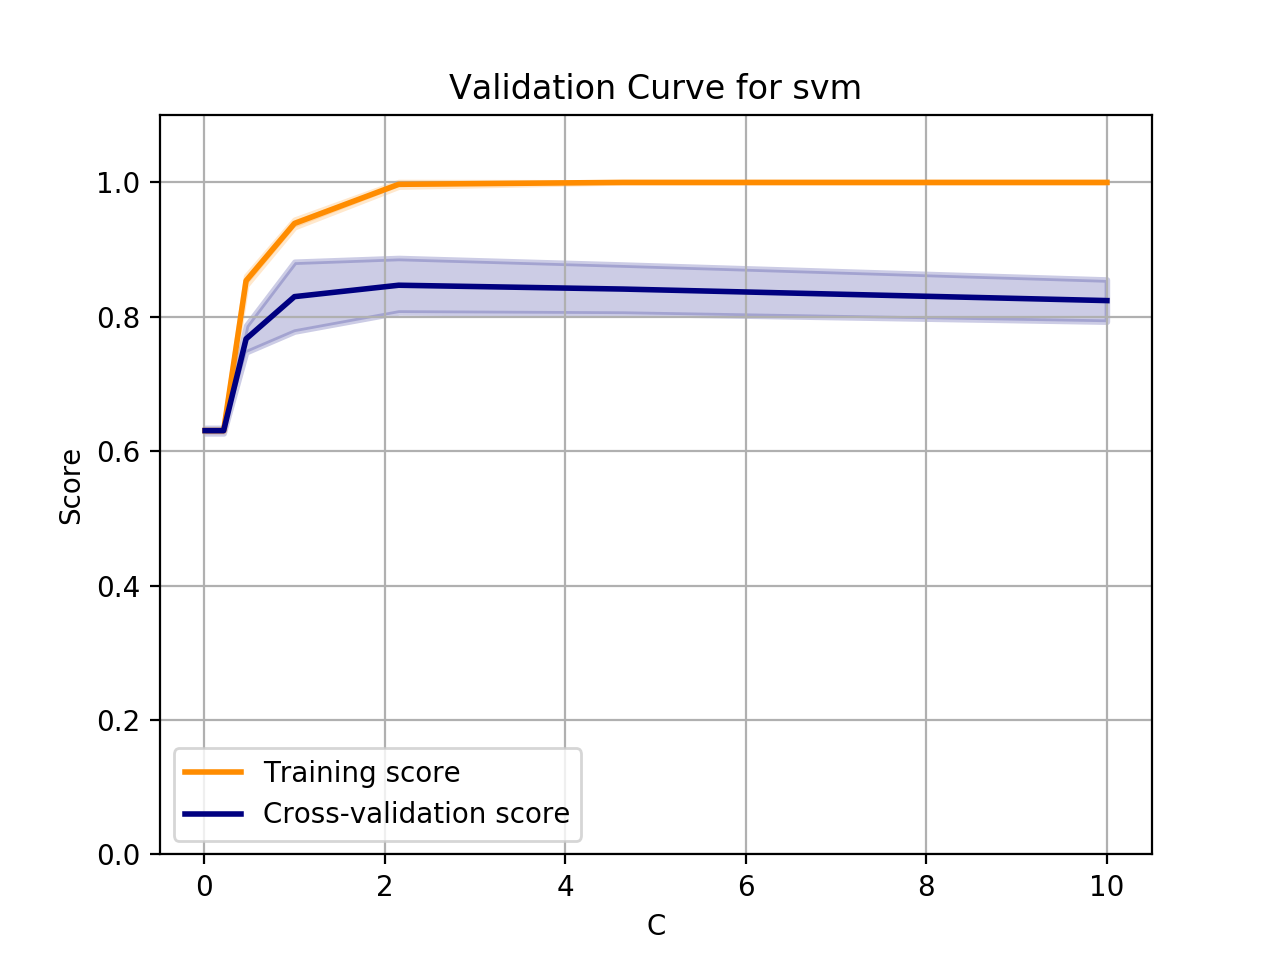
\includegraphics[scale=0.26]{validation_curve}
\caption{SVM learning and validation curves from LPF+HPF processing.}
\end{figure}

Other than SVM, kNN and NN classifiers are used in this project. Even though kNN performed worse than SVM, it is important to state kNN still had some high accuracy values for equalized version of images. With LPF+HPF, kNN was able to beat the 85\% accuracy threshold and showed promising results. LPF+HPF worked very well for kNN as LPF+HPF almost created binary images with brain tissues and a nearest-neighbor approach was able to detect the tumor very well. We believe the other filtering techniques did not work well with kNN because there were too much detail in those images compared to LPF+HPF. For kNN classifier, after using cross-validation, 7 nearest neighbors are used as the k parameter. It is important to note that, the number of neighbors did not affect the accuracy results significantly, as a weighted distance approach is used and some imaging filters outputted complex images. Without weighted distance approrach, the accuracy results turned out to be lower. At the end, we still argue that kNN classifier can be used for tumor identification when certain image processing techniques such as LPF+HPF is used. 

Finally, NN classifier also showed worse results, which was interesting. We argue that lack of training data caused this performance. It is also observed that different sigma values or different image filters did not help with the accuracy values that much, as the NN classifier itself just showed bad performance with the given data. The NN classifier was also optimized using cross validation. An adaptive learning rate and ReLU activation function is selected for the Neural Network. Even though our NN showed low accuracy results, we believe a Convolutional Neural Network (CNN) approach should also be considered for future experiments. However, with limited training data, it would be hard to get high accuracies with any type of neural network.  

After analyzing all our experimental results of validation accuracies, we created our final classifier that is based on ensemble learning. We chose SVM as the dominant classifier and selected the best image filter/sigma combinations. We chose ensemble learning approach to combat with overfitting of SVM classifier and to generalize the limited training data. By using different image filters, we tried to solve the classification problem by focusing on different parts of the image, such as high frequency content or brain tissue. At the end, ensemble learning turned out to be very helpful to reduce overfitting and increase generalization. The final confusion matrix of our final classifier is shown in Figure 10. The matrix suggests that ensemble classifier outputted an accuracy value of 87\% and a false negative rate of 2\%. Hence, we observe that ensemble learning was helpful to increase accuracy and to minimize the number of false negatives. Finally, Table IV shows the computation time of our final classifier. In less than 40 seconds, our final classifier can be trained for high accuracy. Additionally, given an MRI scan, our classifier can predict whether it has a tumor or not in only 8 seconds. 

\begin{figure}[h]
\centering
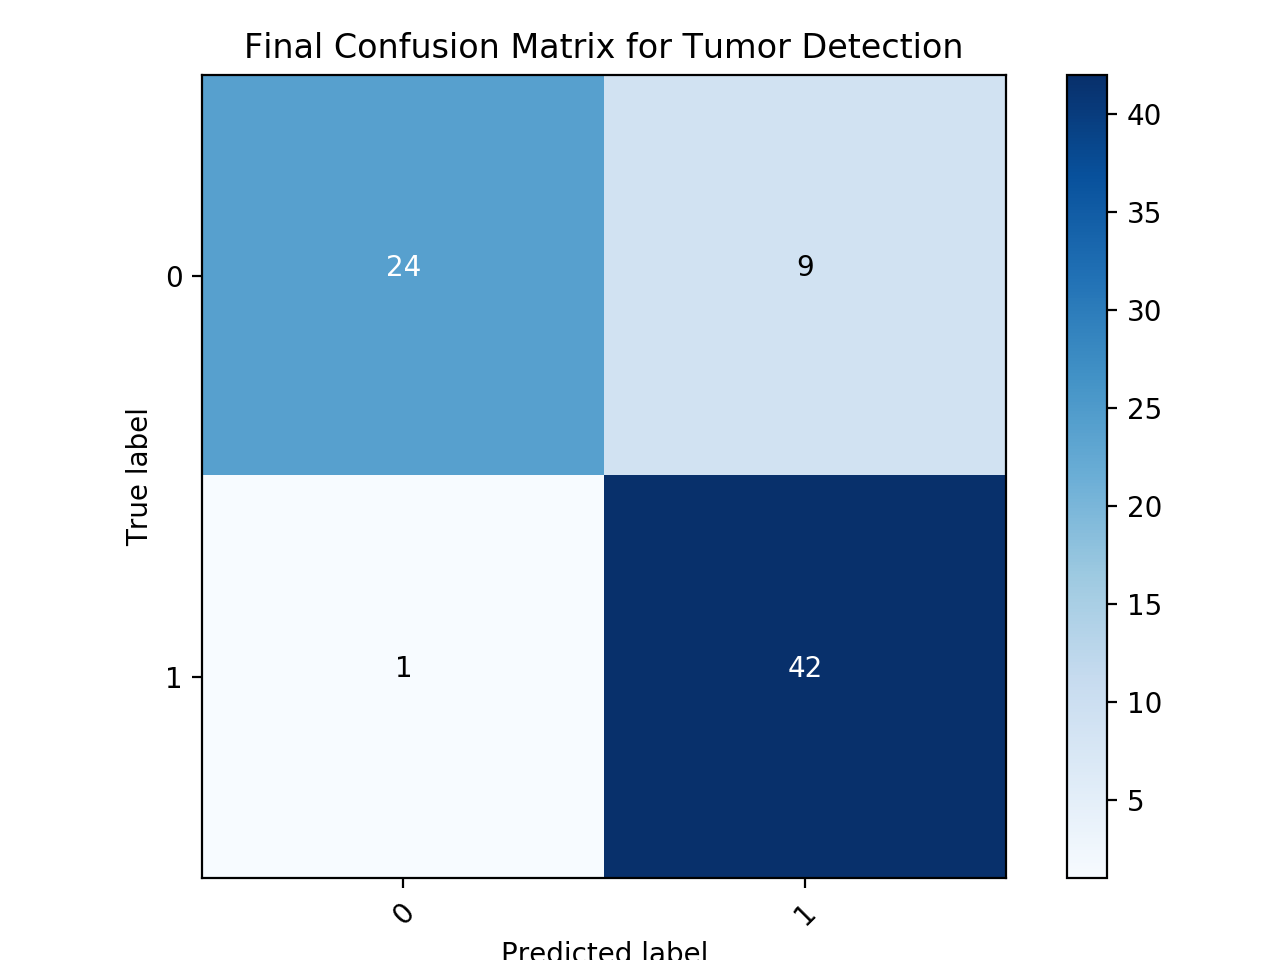
\includegraphics[scale=0.35]{final_confusion_matrix}
\caption{Final confusion matrix from our ensemble learning classifier.}
\end{figure}

\begin{table}[h]
\centering
\caption{Training and inference time of our final classifier. }
\label{tab:my-table}

\begin{tabular}{|l|c|}
\hline
          & \multicolumn{1}{l|}{Computation Time (s)} \\ \hline
Training  & 39                                        \\ \hline
Inference & 8                                         \\ \hline
\end{tabular}
\end{table}

At the end, when our final classifier is analyzed, it is important to note the low rate of false negatives. We argue that the false negative rate is more significant than our final accuracy value in the domain of healthcare. For brain tumor identification, a high accuracy with a high number of false negatives can still cause devastating results for patients and might be life threatening. Hence, we argue that our contribution to brain tumor identification is significant as our classifier almost always benefits the health and treatment of the patient. We believe our classifier can be used by physicians to enhance their decision making process.  

% Learning curves, validation curves
% Final Confusion Matrix
% Analyze the results for each filter, different sigma values, and for each ML algorithm
% Which image filter worked the best? --> LPF+HPF analyze other ones too
% Which ML algorithm worked the best? --> SVM analyze other ones too --> why did NN not do good? 
% How helpful was ensemble learning? Why --> generalization
% Discuss false negatives and accuracy 

\section{Conclusion and Future Work}\label{conclusion}
% Briefly summarize main ideas of project --> Best image filter, best classifier, false negatives etc. 
% Discuss future work such as tumor segmentation


\begin{thebibliography}{00}
\bibitem{b1} Hallberg Ö, Morgan LL (2011) The Potential Impact of Mobile Phone Use on Trends in Brain and CNS Tumors. J Neurol Neurophysiol S5. doi:10.4172/2155-9562.S5-003
\bibitem{b2} Australian Institute of Health and Welfare 2019. Cancer in Australia 2019. Cancer series no.119. Cat. no. CAN 122. Canberra: AIHW.
\bibitem{b3} Gamage, Praveen. (2017). Identification of Brain Tumor using Image Processing Techniques. 
\bibitem{b4} Gaikwad, Sonali \& Joshi, M.. (2015). Brain Tumor Classification using Principal Component Analysis and Probabilistic Neural Network. International Journal of Computer Applications. 120. 5-9. 10.5120/21205-3885.
\bibitem{b5} Ari, Ali \& Hanbay, Davut. (2018). Deep learning based brain tumor classification and detection system. TURKISH JOURNAL OF ELECTRICAL ENGINEERING \& COMPUTER SCIENCES. 26. 2275-2286. 10.3906/elk-1801-8.
\bibitem{b6} Seetha, J. \& Raja, S.. (2018). Brain Tumor Classification Using Convolutional Neural Networks. Biomedical and Pharmacology Journal. 11. 1457-1461. 10.13005/bpj/1511. 
\bibitem{b7} Kernick DP, Ahmed F, Bahra A, et al. Imaging patients with suspected brain tumour: guidance for primary care. Br J Gen Pract. 2008;58(557):880–885. doi:10.3399/bjgp08X376203.
\end{thebibliography}

\end{document}
